Data

\subsection{Data Description and Initial Sampling}
\label{sec:datadescription}



\newpage

\subsection{Dimensionality Reduction}
\label{sec:dimred}

Model training over high-dimensional parameter spaces may be facilitated by carefully reducing the number of variables used to describe the space. For many applications, feature selection strategies succeed in identifying a sufficiently representative subset of the original input variables; however, all given variables were assumed to be physically relevant to the MC TBR model. Feature extraction methods, on the other hand, aim to identify a transformation from the parameter space which decreases dimensionality; even if no individual parameter is separable from the space, some linear combinations of parameters or nonlinear functions of parameters may be.

\begin{figure}[h]
  \centering
    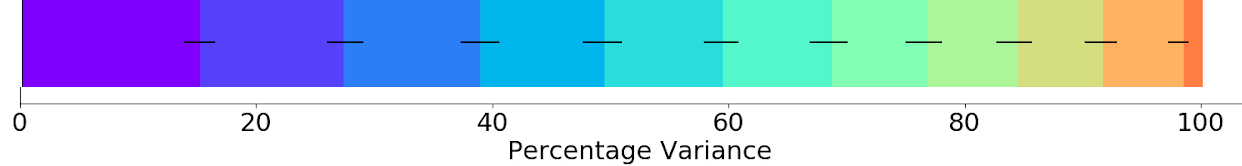
\includegraphics[width=0.6\linewidth]{fig2_pca.jpg}
    \caption{Cumulative variance for optimal features identified by PCA}
  \label{fig:pca}
\end{figure}

\begin{wrapfigure}{r}{0.5\textwidth}
  \vspace{-55pt}
  \begin{center}
    \hspace*{-.3\columnsep}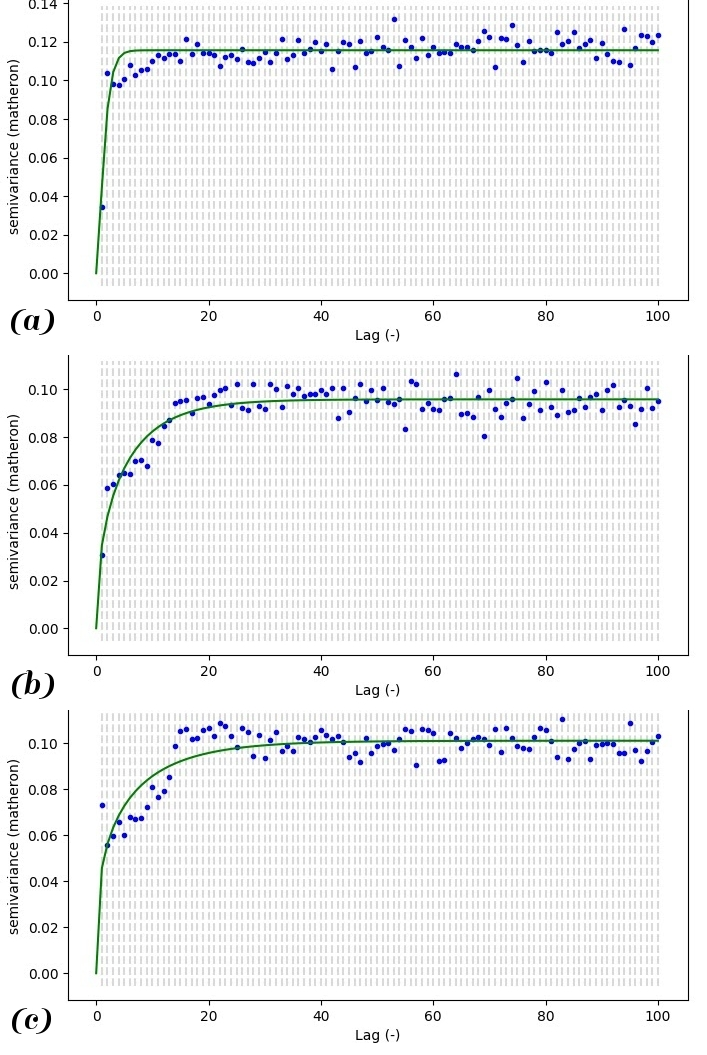
\includegraphics[width=0.58\textwidth]{fig3_allvar.jpg}
    \caption{Semivariograms for MC TBR data with coolant materials: (a) $He$, (b) $H_2O$, (c) $D_2O$}
    \label{fig:var}
  \end{center}
  \vspace{-110pt}
\end{wrapfigure}

\subsubsection{Principal Component Analysis}

To pursue linear feature extraction, principal component analysis (PCA) was performed via scikit-learn on a set of 300,000 uniform samples of the MC TBR model. 

Figure \ref{fig:pca} shows the resultant cumulative variance of the feature vectors identified by PCA. The similar share of variance among all eleven features demonstrated irreducibility of the TBR model by linear methods.

\subsubsection{Variogram Computations}

Kriging, or Gaussian process regression, is a geostatistical surrogate modelling technique which relies on correlation functions over distance (lag) in the paramater space [2]. Although kriging performed poorly for our use case due to high dimensionality, these correlation measures gave insight into similarities between discrete-parameter slices of the data.

Figure \ref{fig:var} shows the Matheron semivariance [3] for three discrete slices with coolant material varied, but all other discrete parameters fixed. Fits [4] to the Matérn covariance model confirmed numerically that the coolant material is the discrete parameter with the greatest distinguishability in the MC TBR model. 


** Make sure discrete slices are mentioned before this **

\subsubsection{Autoencoders}

Question: is it accurate to say this represents nonlinear feature extraction? re my intro paragraph

\newpage
